%-----------------------------------------------------------------------------------------------
\makeatletter
\immediate\write18{datelog > \jobname.info} % site script for $(date '+%Y-%m-%d %Hh%Mm%Ss')
\makeatother
%-----------------------------------------------------------------------------------------------
%-----------------------------------------------------------------------------------------------
\usetheme{Copenhagen}
\usepackage{beamercolorthemeCNThermSci2}
\usefonttheme{serif}
%-----------------------------------------------------------------------------------------------

%-----------------------------------------------------------------------------------------------
%-----------------------------------------------------------------------------------------------
\usetheme{Copenhagen}
\usepackage{beamercolorthemeUTF2}
\usefonttheme{serif}
%-----------------------------------------------------------------------------------------------
\usepackage[utf8]{inputenc}
\usepackage[greek,french,english,brazil]{babel} % last becomes the active one
\usepackage{pslatex}
\usepackage{amssymb,amsmath}
\usepackage{soul}
\usepackage[squaren,Gray,cdot]{SIunits}
\usepackage[nice]{nicefrac}
\usepackage{tikz}
\usepackage{amscd}
\usepackage{stmaryrd}
\usepackage{scalerel}
\usepackage{xspace}
%-----------------------------------------------------------------------------------------------


%-----------------------------------------------------------------------------------------------
%-----------------------------------------------------------------------------------------------
% Mathematical
%-----------------------------------------------------------------------------------------------
\newcommand{\vet}[1]{\underline{{#1}}}
\newcommand{\mat}[1]{\underline{\underline{{#1}}}}
\newcommand{\cub}[1]{\underline{\underline{\underline{{#1}}}}}
\newcommand{\eqdef}{{\ensuremath\stackrel{\text{\tiny def}}{=}}}
%-----------------------------------------------------------------------------------------------
% Linguistic
%-----------------------------------------------------------------------------------------------
\newcommand{\GRtxt}[1]{\begin{otherlanguage}{greek}{{#1}}\end{otherlanguage}}
\newcommand{\FRtxt}[1]{\begin{otherlanguage}{french}{{#1}}\end{otherlanguage}}
%-----------------------------------------------------------------------------------------------
% Presentation
%-----------------------------------------------------------------------------------------------
\newcommand{\BkgImgH}[1]{% Places an image centered on the slide background filling the height
    \usebackgroundtemplate{\parbox{\paperwidth}{%
        \vspace*{1sp}\centering\includegraphics[height=\paperheight]{{#1}}
}}}
\newcommand{\BkgImgW}[1]{% Places an image centered on the slide background filling the width
    \usebackgroundtemplate{\parbox{\paperwidth}{%
        \vspace*{1sp}\centering\includegraphics[width=\paperwidth]{{#1}}
}}}
\newcommand{\ArtEndH}[3]{% Transitions to plain image (last) slide: #1:prefix #2,#3:extensions
    \BkgImgH{root/../art/#1.#2}
    \frame<handout:0>[plain]{%
        \transdissolve\vspace*{72mm}\color{white}\scriptsize\bf\input{root/../art/#1.#3}}
    \usebackgroundtemplate{\mbox{~}}
}
\newcommand{\ArtEndW}[3]{% Transitions to plain image (last) slide: #1:prefix #2,#3:extensions
    \BkgImgW{root/../art/#1.#2}
    \frame<handout:0>[plain]{%
        \transdissolve\vspace*{72mm}\color{white}\scriptsize\bf\input{root/../art/#1.#3}}
    \usebackgroundtemplate{\mbox{~}}
}
\newcommand{\ImgColW}[3]{% Inserts a full-width image in a column
    \includegraphics[width=\columnwidth]{root/../art/#1.#2}\\[-0.5\baselineskip]
    \parbox{\columnwidth}{\tiny\hfill\scalebox{0.85}{\input{root/../art/#1.#3}}}
}
\newcommand{\txtpic}[1]{%
    \fcolorbox{lightgray}{white!90!black}{{#1}} 
}
%-----------------------------------------------------------------------------------------------


%-----------------------------------------------------------------------------------------------
\title{A.03.02 -- Processos Politrópicos}
\subtitle{(Sistemas Fechados)}
\author{Prof.~C.~Naaktgeboren, PhD}
\date{{\scriptsize\tt%
    
\includegraphics[height=6.0mm]{root/00-res/cc/by-nc-nd-88x31.pdf}\\[\smallskipamount]
    https://github.com/CNThermSci/ApplThermSci\\
    Compiled on \input{\jobname.info}
}}
%-----------------------------------------------------------------------------------------------
\begin{document}
%-----------------------------------------------------------------------------------------------
\logo{%
    \parbox{158mm}{% There's a 1mm gap on each side of the 160mm x 90mm slide logo line
        \mode<beamer>{
            
\includegraphics[height=6.0mm]{root/00-res/UTFPR/UTFPR-logo-D.pdf}\hfill%
            
\includegraphics[height=9.0mm]{root/00-res/logo/CNThermSci-logo-A.pdf}%
        }
        \mode<handout>{
            
\includegraphics[height=6.0mm]{root/00-res/UTFPR/UTFPR-logo-W.pdf}\hfill%
            
\includegraphics[height=9.0mm]{root/00-res/logo/CNThermSci-logo-W.pdf}%
        }
    }
} % The (delineated, alpha), or washed-out logos
%-----------------------------------------------------------------------------------------------
\frame{\titlepage}
%-----------------------------------------------------------------------------------------------

%-----------------------------------------------------------------------------------------------
\section*{Sumário Geral}
%-----------------------------------------------------------------------------------------------

%-----------------------------------------------------------------------------------------------
\subsection{Parte~I: Apresentação de Processo Politrópico}
%-----------------------------------------------------------------------------------------------

\frame<handout:0>{
    \frametitle{Sumário da Parte~I}
    \tableofcontents[part=1]
}

%-----------------------------------------------------------------------------------------------
\subsection{Parte~II: Tópicos Especiais em Processos Politrópicos}
%-----------------------------------------------------------------------------------------------

\frame<handout:0>{
    \frametitle{Sumário da Parte~II}
    \tableofcontents[part=2]
}

%===============================================================================================
\part{Apresentação de Processo Politrópico}
\frame<handout:0>{\partpage}
%===============================================================================================

%-----------------------------------------------------------------------------------------------
\section{Processos Politrópicos}
%-----------------------------------------------------------------------------------------------

%-----------------------------------------------------------------------------------------------
\subsection{Apresentação}
%-----------------------------------------------------------------------------------------------

    % !j 96 -i8
    %-------------------------------------------------------------------------------------------
    \begin{frame}{Processos Politrópicos -- Definição}\vspace*{-2em}
        \begin{columns}
        \column{0.50\textwidth}
        É todo o processo para o qual:
        \alert{$$Pv^n = \mbox{const.}$$}%
        \uncover<5->{%
            \par\noindent A equação é utilizada na forma:
            $$P_1v_1^n = P_2v_2^n.$$%
        }%
        \uncover<6->{%
            \par\noindent A versão \alert{$PV^n = \mbox{const.}$}, também é usual.
        }
        \column{0.50\textwidth}
        \uncover<2->{Onde:} \\[\bigskipamount]
        \begin{itemize}
            \item<2-> $P$ é a pressão do sistema \\[\bigskipamount]
            \item<3-> $v$ é o volume específico do sistema \\[\bigskipamount]
            \item<4-> $n$ é o \alert{expoente politrópico}
        \end{itemize}
        \end{columns}
    \end{frame}
    %-------------------------------------------------------------------------------------------

    % !j 96 -i8
    %-------------------------------------------------------------------------------------------
    \begin{frame}{Processos Politrópicos -- Apresentação}\vspace*{-2em}
        Em processos politrópicos, \\[\medskipamount]
        \begin{itemize}
            \item<1-> um \alert{parâmetro} de processo, \alert{$n$}, é mantido constante
                \\[\medskipamount]
            \item<2-> e não \alert{necessariamente} uma \alert{propriedade} do sistema.
                \\[\medskipamount]
            \item<3-> porém uma propriedade \alert{pode} ficar constante, como veremos.
                \\[\bigskipamount]
        \end{itemize}
        \uncover<4->{Um exemplo trivial é reconhecer que para \alert{$n = 0$}, tem-se:}
        \uncover<5->{$$Pv^0 = \mbox{const.} \rightharpoondown\quad \alert{P = \mbox{const.}}$$}
    \end{frame}
    %-------------------------------------------------------------------------------------------

    % !j 96 -i8
    %-------------------------------------------------------------------------------------------
    \begin{frame}{Processos Politrópicos -- Apresentação}\vspace*{-2em}
        \begin{align*}
            \uncover<3->{\log\big(}
            Pv^n & \only<1>{= \mbox{const.}}\uncover<2->{= c_1}
            \uncover<3->{\big)\rightharpoondown} \\[\medskipamount]
            \uncover<4->{
                \log(Pv^n) & = \log(c_1) \equiv c_2 \rightharpoondown \\[\medskipamount]
            }
            \uncover<5->{
                \log P + n\log v & = c_2 \rightharpoondown \\[\medskipamount]
            }
            \uncover<6->{
                \log P & = c_2 - n\log v
                \uncover<7->{\qquad\therefore\qquad\mbox{uma equação na forma}}
                \\[\medskipamount]
            }
            \uncover<8->{
                \alert{y} & \alert{= A + Bx}\qquad
                \mbox{para $y\equiv\log{P}$, $\quad x\equiv\log{v},\quad$ etc.}
            }
        \end{align*}
    \end{frame}
    %-------------------------------------------------------------------------------------------

    % !j 96 -i8
    %-------------------------------------------------------------------------------------------
    \begin{frame}{Processos Politrópicos -- Apresentação}\vspace*{-2em}
        \begin{columns}
        \column{0.55\textwidth}
        Assim:
        \begin{itemize}
            \item \alert{Todo} processo \alert{politrópico} \\[\medskipamount]
            \item é representado por um \alert{segmento de reta} \\[\medskipamount]
            \item que une os estados \alert{inicial} e \alert{final} \\[\medskipamount]
            \item em coordenadas \alert{$\log P \times \log v$}. \\[\medskipamount]
        \end{itemize}
        \uncover<2->{%
            \noindent Logo, processos politrópicos a $\alert{v = \mbox{const.}}$, são obtidos
            fazendo \alert{$n \to \pm\infty$}.
        }
        \column{0.45\textwidth}
            \begin{figure}
                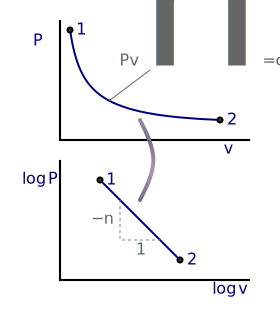
\includegraphics[width=5.0cm]{fig/A0302-pt-PolyProcPlotPv.pdf}
            \end{figure}
        \end{columns}
    \end{frame}
    %-------------------------------------------------------------------------------------------

    % !j 96 -i8
    %-------------------------------------------------------------------------------------------
    \begin{frame}{Processos Politrópicos -- Etimologia}\vspace*{-2em}
        Segundo (Chantraine, 1968), o termo ``politrópico'': \\[\medskipamount]
        \begin{itemize}
            \item<1-> origina do grego \alert{``\GRtxt{pol'utropoc}''}, o qual é composto de
                \alert{``\GRtxt{pol'uc}''} e de \alert{``\GRtxt{tr'opoc}''}. \\[\medskipamount]
            \item<2-> \alert{``\GRtxt{pol'uc}''} inclui significados de \FRtxt{\og nombreux,
                vaste\fg}, a saber, ``numeroso, vasto''. \\[\medskipamount]
            \item<3-> \alert{``\GRtxt{tr'opoc}''} inclui significados de \FRtxt{\og manière,
                mode\fg}, a saber, ``maneira, modo''. \\[\medskipamount]
            \item<4-> Ou seja: \alert{``muitas formas ou maneiras''}. O termo composto
                \\[\medskipamount]
            \item<5-> \alert{``\GRtxt{pol'utropoc}''} inclui significados de \FRtxt{\og souple,
                très varié\fg}: ``flexível, muito variado'', \\[\medskipamount]
            \item<6-> indicando \alert{flexibilidade} e a vasta \alert{variedade} de processos
                que pode representar!
        \end{itemize}
    \end{frame}
    %-------------------------------------------------------------------------------------------

%-----------------------------------------------------------------------------------------------
\subsection{Trabalho de Fronteira}
%-----------------------------------------------------------------------------------------------

    % !j 96 -i8
    %-------------------------------------------------------------------------------------------
    \begin{frame}{Processos Politrópicos -- Trabalho de Fronteira}\vspace*{-2em}
        \begin{columns}
        \column{0.40\textwidth}
        \begin{align*}
            \uncover<1->{
                Pv^n & = c_1
                \uncover<2->{= P_1v_1^n = P_2v_2^n \rightharpoondown}
                \\[\medskipamount]
            }
            \uncover<3->{
                P & = c_1v^{-n}; \\[\medskipamount]
            }
            \uncover<4->{
                w_f & = \int_1^2 P\,dv \rightharpoondown \\[\medskipamount]
            }
            \uncover<5->{
                w_f & = c_1 \int_1^2 v^{-n}\,dv \rightharpoondown \\[\medskipamount]
            }
            \uncover<6->{
                w_f & = P_1v_1^n \int_1^2 v^{-n}\,dv.
            }
        \end{align*}
        \column{0.60\textwidth}
        \uncover<7->{A integração de $v^{-n}$ toma formas diferentes dependendo se $n=1$ ou
            não: \\[\medskipamount]
        }
        \begin{equation*}
            \uncover<8->{\alert{
            w_f = \left.\begin{cases}
                \displaystyle\frac{P_2v_2 - P_1v_1}{1-n} & \text{para $n \neq 1$},
                    \\[\bigskipamount]
                Pv \ln\left(\displaystyle\frac{v_2}{v_1}\right) & \text{para $n = 1$}.
            \end{cases}\right.
            }}
        \end{equation*}
        \uncover<9->{%
            \par\noindent No último caso, o produto \alert{$Pv$} pode ser tanto \alert{$P_1v_1$}
            ou \alert{$P_2v_2$}, em função do próprio processo.
        }
        \end{columns}
    \end{frame}
    %-------------------------------------------------------------------------------------------

    % !j 96 -i8
    %-------------------------------------------------------------------------------------------
    \begin{frame}{Processos Politrópicos -- Trabalho de Fronteira -- Gases Ideais}\vspace*{-2em}
        \begin{columns}
        \column{0.45\textwidth}
        \uncover<1->{
            \par\noindent Para gases ideais, \alert{$Pv = RT$}, passando por um processo
            politrópico, \alert{$Pv^n = \mbox{const.}$}, o resultado
        }
        \begin{equation*}
            \uncover<1->{
            w_f = \left.\begin{cases}
                \displaystyle\frac{P_2v_2 - P_1v_1}{1-n} & \text{para $n \neq 1$},
                    \\[\bigskipamount]
                Pv \ln\left(\displaystyle\frac{v_2}{v_1}\right) & \text{para $n = 1$}.
            \end{cases}\right.
            }
        \end{equation*}
        \uncover<2->{
            \par\noindent é válido, mas pode ser escrito como: %\\[\medskipamount]
        }
        \column{0.55\textwidth}
        \begin{equation*}
            \uncover<3->{\alert{
            w_f = \left.\begin{cases}
                \displaystyle\frac{R(T_2 - T_1)}{1-n} & \text{para $n \neq 1$},
                    \\[\bigskipamount]
                Pv \ln\left(\displaystyle\frac{v_2}{v_1}\right) & \text{para $n = 1$}.
            \end{cases}\right.}\text{(gás ideal)}
            }
        \end{equation*}
        \uncover<4->{
            \par\noindent Para \alert{gases ideais}, expoente \alert{$n=1$} significa:
        }
        \uncover<5->{
            $$Pv^1 = \mbox{const.} = RT \quad\rightharpoondown\quad \alert{T = \mbox{const.}}$$
        }
        \end{columns}
    \end{frame}
    %-------------------------------------------------------------------------------------------

%-----------------------------------------------------------------------------------------------
\section{Tópicos de Leitura}
%-----------------------------------------------------------------------------------------------

    %------------------------------------------------------------------------------------------
    \begin{frame}[allowframebreaks]{Tópicos de Leitura}
        \begin{thebibliography}{Çengel, Y.~A., 2013}
            \bibitem[Çengel, Y.~A., 2013]{2013-CengelYA+BolesMA-AMGH}
                Çengel, Y.~A. e Boles, M.~A.
                \newblock{{\em Termodinâmica $7^\mathrm{a}\!$ Edição\/}. \alert{Seção~4-1.}}
                \newblock{\footnotesize AMGH. Porto Alegre. ISBN 978-85-8055-200-3.}
        \end{thebibliography}
    \end{frame}
    %------------------------------------------------------------------------------------------

    % Finishes with stunning image, with credit
    \ArtEndWSE{pexels-nuno-obey-127160}{jpg}{txt}

%===============================================================================================
\part{Tópicos Especiais em Processos Politrópicos}
\frame<handout:0>{\partpage}
%===============================================================================================

%-----------------------------------------------------------------------------------------------
\section{Tópicos Especiais em Processos Politrópicos}
%-----------------------------------------------------------------------------------------------

    % !j 96 -i8
    %-------------------------------------------------------------------------------------------
    \begin{frame}{Tópicos Especiais em Processos Politrópicos -- Pré-Requisitos}\vspace*{-2em}
        Os tópicos especiais em processos politrópicos têm por pré-requisito:
        \begin{itemize}
            \item A \alert{primeira lei da Termodinâmica}; \\[\medskipamount]
            \item O \alert{balanço de energia}; e \\[\medskipamount]
            \item \alert{Propriedades energéticas} de gases ideais. \\[\bigskipamount]
        \end{itemize}
        Que constituem o tópico \texttt{A0303} desta série.
    \end{frame}
    %-------------------------------------------------------------------------------------------

%-----------------------------------------------------------------------------------------------
\subsection{Fundamentação Teórica}
%-----------------------------------------------------------------------------------------------

    % !j 96 -i8
    %-------------------------------------------------------------------------------------------
    \begin{frame}{Tópicos Especiais -- Fundamentação Teórica}\vspace*{-2em}
        \uncover<1->{Tomando-se a $1^{\mathrm{a}}$ lei na forma diferencial e:}
        \begin{itemize}
            \item<2-> definindo a \alert{razão de calor e trabalho}, $K \equiv \frac{\delta
                q}{\delta w}$, \\[\medskipamount]
            \item<3-> também conhecida como \alert{razão de transferência de energia},
                \\[\medskipamount]
            \item<4-> e substituindo no balanço de energia na forma direfencial, tem-se:
                \\[\medskipamount]
        \end{itemize}
        \begin{align*}
            \uncover<5->{
                \delta{q} - \delta{w} & = du \qquad\rightharpoondown
                \\[\medskipamount]
            }
            \uncover<6->{
                (K-1)\delta{w} & = du \qquad\rightharpoondown
                \\[\medskipamount]
            }
            \uncover<7->{
                (K-1)P\,dv & = du.
                %\\[\medskipamount]
            }
        \end{align*}
    \end{frame}
    %-------------------------------------------------------------------------------------------

    % !j 96 -i8
    %-------------------------------------------------------------------------------------------
    \begin{frame}{Tópicos Especiais -- Fundamentação Teórica (cont.)}\vspace*{-2em}
        \uncover<1->{Assumindo comportamento ideal da substância que compõe o sistema:}
    \end{frame}
    %-------------------------------------------------------------------------------------------

%-----------------------------------------------------------------------------------------------
\subsection{Processos Localmente Politrópicos}
%-----------------------------------------------------------------------------------------------

    % !j 96 -i8
    %-------------------------------------------------------------------------------------------
    \begin{frame}{Tópicos Especiais -- Processos Localmente Politrópicos}\vspace*{-2em}
        A SER CONTINUADO PARA A PARTE-II...
    \end{frame}
    %-------------------------------------------------------------------------------------------

%-----------------------------------------------------------------------------------------------
\section{Tópicos de Leitura}
%-----------------------------------------------------------------------------------------------

    %------------------------------------------------------------------------------------------
    \begin{frame}[allowframebreaks]{Tópicos de Leitura}
        \begin{thebibliography}{Çengel, Y.~A., 2013}
            \bibitem[Çengel, Y.~A., 2013]{2013-CengelYA+BolesMA-AMGH}
                Çengel, Y.~A. e Boles, M.~A.
                \newblock{{\em Termodinâmica $7^\mathrm{a}\!$ Edição\/}. \alert{Seção~4-1.}}
                \newblock{\footnotesize AMGH. Porto Alegre. ISBN 978-85-8055-200-3.}
        \end{thebibliography}
    \end{frame}
    %------------------------------------------------------------------------------------------

    % Finishes with stunning image, with credit
    \ArtEndW{pexels-brandon-montrone-1374295}{jpg}{txt}

%-----------------------------------------------------------------------------------------------
\end{document}
%-----------------------------------------------------------------------------------------------

